\chapter{Implementation}
\label{cha:implementation}

The final implementation of our system was follows:
\begin{figure}[h]
\centering
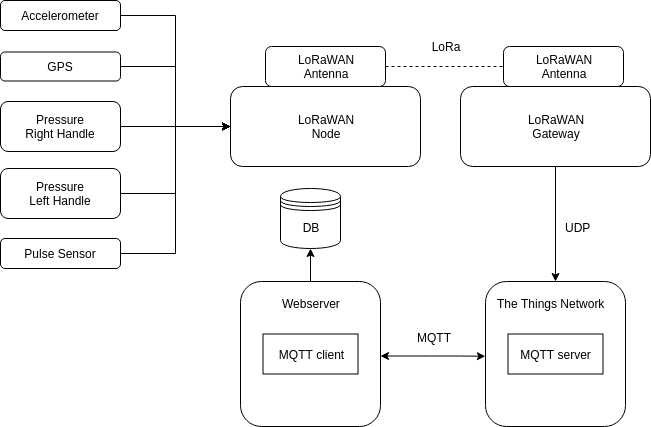
\includegraphics[width=0.7\linewidth]{gfx/implementation_arch}
\caption[]{Implemented Architecture}
\label{fig:implementation_arch}
\end{figure}

It differed from the overall design in the following ways:

We decided to use a webserver with an mqtt client and a database instead of a central server with API. We also decided to not implement the analytics server as part of the current project. We made these decisions prioritising the components that we needed to test our hypothesis. Since the presence or absence of a central server or analytics platform don't affect the parameters we need to test our hypothesis we decided to ignore them in the implementation part.

The implementation of each component of our system is described in details in the following subsections.



\subsection{Node:} 

\subsubsection{Hardware:}
The node consists of an Arduino Mega (R3 ATmega2560) with a Seeedstudio Dragino Lora Shield (868 M Frequency). The node is powered by a standard 9V battery pack. The node also consists of a breadboard, which contains two Analog to Digital converter and a gps sensor. The entire node setup is mounted on the front face of the lower left leg of the walker. The accelerometer is directly connected to the arduino and is mounted on the back face of the left leg of walker. Two pressure sensors are mounted on the handles of the walker and are connected to the A/D converters in the breadboard, which in turn are connected to the arduino. The pulse sensor is mounted on the left handle and is on top of a button and is directly connected to the arduino. The pulse sensor is only activated if the underlying button is pressed. 

The circuit diagram of the node is as follows:



\subsubsection{Software:}
The IDE used for writing and uploading the code was Visual Studio with Platform I/O extension. The Platform I/O simplified the process of uploading the code and monitoring the output of the arduino mega.

The libraries used were lmic, hal, SPI, SoftwareSerial, MPU9250 and HX711 along with the standard Arduino,stdlib and string library.

The code structure is as follows:
--Insert code tree here---

The main.cpp collects data in case of an event, converts the said data to bytes and sends it to a gateway using LoRaWAN. The main calls sensor specific functions to collect the data. 

Each LoRa packet contains the application id and key that is required by the things network.

\subsection{Pressure:}

\subsubsection{Hardware:}
For measuring pressure we used two 10kg Aluminum Alloy pressure sensors connected to the Arduino via a HX711 AD converter module. 

\subsubsection{Software:}
The sensor data was collected using HX711 library to transform the analog signal along with standard Arduino library. 

\subsection{Pulse:}


\subsection{Hardware:}
For pulse, we used the pulse sensor from pulsesensor.com.


\subsubsection{Software:}
For reading the data from the sensor, simple analog read was used. This data is then processed to get average heart rate of the patient by looking at the heardbeat pattern.



\subsection{Accelerometer:}

\subsection{Hardware:}
We used an MPU9250 accelerometer to measure whether the walker is moving or not.

\subsubsection{Software:}
The library used to read the accelerometer's output was sensor specific MPU9250 library. If the gyroscope reading from the accelerometer increased beyond a certain threshold, the walker was considered to be moving.


\subsection{GPS:}

\subsection{Hardware:}
For measuring GPS we used the GY-GPS6MV2 sensor.

\subsubsection{Software:}
The library used to read GPS data was SoftwareSerial. The read data was parsed to get the value of latitude and longitude, which were then converted to bytes.



\subsection{Gateway:}

\subsection{Hardware:}
We used raspberry pi 3+ along with dragino lora hat with gps model number 979854 for the gateway.
The gateway was made of a Raspberry Pi 3+ with a Dragino LoRa hat for Pi. The Pi was connected to a router which in turn was connected to the internet.


The circuit layout of the gateway is





\subsubsection{Software:}
the pi has a single chain packet forwarder code written in c, which forwards the packets it receives from the node to The Things Network's IP address. 


\subsection{The Things Network (TTN):}
The things network is an online website that we used to host our mqtt broker. We chose TTN because it's convinient, secure and very popular among the LoRaWAN community. We created an application in the TTN to act as our mqtt broker. We laso registered our gateway in TTN.

The application in TTN received packets from the gateway, converted them back from byte string to json and published them using the mqtt broker.


\subsection{Webserver:}
We created a webserver using the Django framework. It contained an mqtt client which subscribed to TTN. The mqtt borker was implemented using the paho mqtt library. The server then parsed the received data and stored them in a sqlite database. The database was then queried and the result was displayed on a webpage using django-tabular library.

We chose Django with sqlite for our server, because they allow quick prototyping and testing.

%%% Local Variables:
%%% mode: latex
%%% TeX-master: "../ClassicThesis"
%%% End:
